\section{System Design}

  In this section, we describe the design of Lever. Lever is designed to be API-compatible with the original system, providing the mitigation transparency and developer transparency. We begin with an overview of the system architecture, followed by introducing the system details.

\subsection{System Overview}

  Figure 4 overviews the architecture of Lever. Lever periodically collects and analyzes the historical jobs' profiles of recurring batch streaming jobs. Based on these analysis, Lever pre-schedules job input data through three main steps, i.e. identify potential stragglers, evaluate nodes' capability and choose suitable helpers. Firstly, comparing each node's task finish time in previous batch, Lever can initially determine initial state of each node. Lever also estimates the tendency of input load. Combined with these two aspects, Lever conduct state transition to decide which nodes will behaviors as stragglers in next batch(for Challenge 1). Secondly, based on the fact that batch stream processing jobs are repetitive and periodic, Lever introduces Iterative Learning Control (ILC \cite{Arimoto}), which is designed to do tracking control for systems that work in a repetitive mode to learn to estimate node's capability (for Challenge 2). Finally, considering that Lever don't have resource utilization view when pre-scheduling, Lever can choose all nodes or two least load nodes in faster group as helpers. Lever can switch between these two strategies adaptively to performance best(for Challenge 3).

  We show the actions timing diagram of Lever in Figure 5. We differentiate pre-scheduling and post-scheduling according to their scheduling timing. Post-scheduling acts when processing but pre-scheduling operates on receiving. As shown in Figure 5, at last batch i.e. $t_1$ to $t_2$, Lever needs to collect and analyze previous jobs' execution information, identify potential stragglers and choose suitable helpers. At this batch i.e. $t_2$ to $t_3$, Lever pre-schedules input data according to prior pre-scheduling plan. When come to next batch i.e. $t_3$ to $t_4$, Lever schedules tasks according to data locality as usual. In the following, we present the details of Lever.
  \begin{figure*}[htbp]
    \centering
    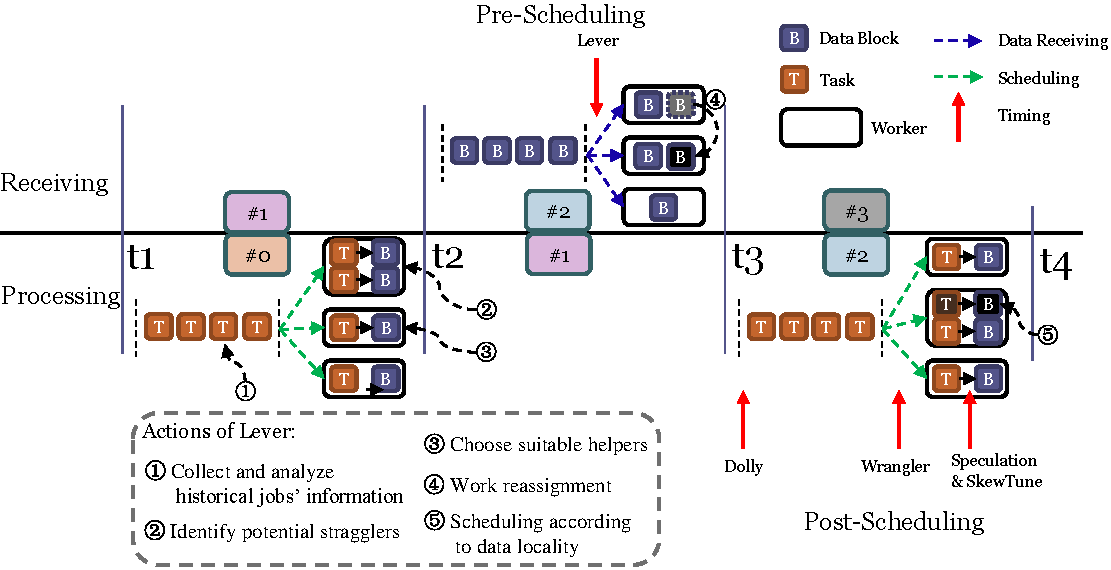
\includegraphics[width=0.75\textwidth]{FigureAction}
    \caption{Actions of Lever}
    \label{Fig. 5:}
  \end{figure*}

\subsection{Identify Potential Stragglers}

  Lever predicts stragglers in the next batch according to recurring jobs' historical execution information combined with the load fluctuation of each node. The first step is to determine the initial stragglers. When last batch's jobs are completed, Lever collects and analyze the statistics of tasks' execution information in each node. The node i's finish time ($NFT_i$) is defined as the time from job's submission to the last task finish in this node. Then, Lever sorts node's list according to $NFT_i$ in the descending order. It classify nodes into three categories according to two locations 0.25, 0.75 of node's list size. Nodes before 0.25$\times$size are grouped into \emph{straggler group}. Nodes after 0.75$\times$size are grouped into \emph{faster group}. The remaining are categorized as \emph{median group}.

  This classification can only represent the stragglers in the last batch and the second step is to add some transition conditions to predict which nodes' state will change in the next batch. First, Lever calculates the median finish time of \emph{straggler group}, \emph{median group} and \emph{faster group} respectively, represented as \emph{FTOS}, \emph{FTOM}, \emph{FTOF}. Second, Lever introduces degradation ratio \emph{FTM} and \emph{MTS}. \emph{FTM} is defined as \emph{FTOM}/\emph{FTOF}. It means that if one node's $NFT_i$ in \emph{faster group} has increased by FTM, it will be moved from \emph{faster group} to \emph{median group} and vice versa. \emph{MTS} is defined as \emph{FTOS}/\emph{FTOM}. It means that if one node's $NFT_i$ in \emph{median group} has increased by MTS, it will be moved from \emph{median group} to \emph{straggler group} and vice versa. We have shown straggler's state transition in Fig. 6.
  \begin{figure}[htbp]
    \centering
    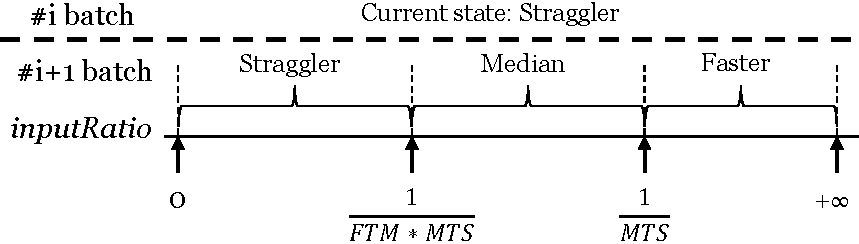
\includegraphics[width=0.42\textwidth]{FigureI2}
    \caption{An example for straggler's state transition}
    \label{Fig. 6:}
  \end{figure}

  The third step is to do state transition, taking the load fluctuation into account. As stream load varies over time, last batch's stragglers may receive much less data and hence become faster in this batch. Also last batch's fasters may receive much more data to be overloaded and it will become straggler in this batch. Lever introduces \emph{inputRatio} as a metric of stream load trend. It is defined as the quotient of new input rate in this batch and old input rate in last batch. We show the transition rules in Table \uppercase\expandafter{\romannumeral1}. Lever applies these rules to each node and decides final stragglers.
  \begin{table}[htbp]
    \footnotesize
    \centering
    \caption{Transition rules for identifying stragglers}
    \begin{threeparttable}
    \centering
      \begin{tabular}{|p{1.5cm}|p{4.3cm}|p{1.4cm}|}
        \hline
        Initial State & Transition Conditions(inputRatio) & Final State \\
        \hline
        \multirow{3}{2cm}{Straggler} &
        (1/MTS,$+\infty$) & Straggler \\
        \cline{2-3}
        & [1/(FTM*MTS),1/MTS] & Median \\
        \cline{2-3}
        & (0,1/(FTM*MTS)) & Faster \\
        \hline
        \multirow{3}{2cm}{Median} &
        (MTS,$+\infty$) & Straggler \\
        \cline{2-3}
        & [1/FTM,MTS] & Median \\
        \cline{2-3}
        & (0,1/FTM) & Faster \\
        \hline
        \multirow{3}{2cm}{Faster} &
        (FTM*MTS,$+\infty$) & Straggler \\
        \cline{2-3}
        & [FTM,FTM*MTS] & Median \\
        \cline{2-3}
        & (0,FTM) & Faster \\
        \hline
      \end{tabular}
    \end{threeparttable}
    \label{Table1}
  \end{table}

\subsection{Computational Capability Determination}

  In order to conduct capability-aware pre-scheduling, Lever evaluates each node's computational capability by leveraging the characteristics of recurring batch stream jobs.

\subsubsection{Computational Capability}

  As shown in Section \uppercase\expandafter{\romannumeral2}-C, recurring batch stream jobs have stable data properties such as computational capability. By analyzing the previous execution, We can assess these metrics exactly in the subsequent execution.

  Considering the periodicity of recurring batch stream jobs, we evaluate computational capability based on a well-known optimization technique, Iterative Learning Control (ILC \cite{Arimoto}), which is designed to do tracking control for systems that work in a repetitive mode. This learning process uses information from previous repetitions to improve the estimation ultimately enabling a more and more accurate result can be found iteratively.
  \begin{figure}[htbp]
    \centering
    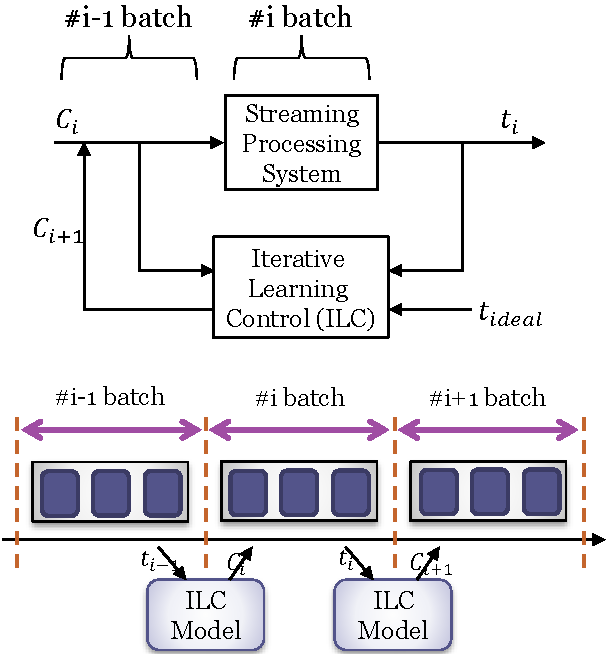
\includegraphics[width=0.36\textwidth]{FigureILC}
    \caption{The principle of evaluating computational capability with ILC.}
    \label{Fig. 7:}
  \end{figure}

  Fig. 7 shows the principle of ILC algorithm. A simple control law for one node is of the following form:
  \begin{equation}
  C_{i+1} = C_i + K*\Delta t
  \end{equation}
   \begin{equation}
  \Delta t = t_{ideal} - t_{i}
  \end{equation}
  where $C_i$ is the input capability to the stream processing system during the ith batch, $\Delta t$ is node's finish time error during the ith batch and K is a design parameter representing operations on $\Delta t$. In Lever, K is set to $C_i/t_i$. $t_{ideal}$ is the ideal node's finish time in the ith batch and can be got by computing the median node's finish time. At beginning, initial $C_{initial}$ is computed as the average of $C_1$, $C_2$ and $C_3$.

\subsubsection{Theoretical Data Assignment}

  In the ideal case, every task should be completed simultaneously. The system should increase the amount of load in faster node and decrease those in straggler to minimize the makespan. Assume that there are n nodes, Let \emph{$L_i$} and \emph{$C_i$} denote the input load and the computational capability of node i respectively. Let \emph{$L_i^\prime$} denote the input load after been tweaked. Let $t_i$ denote the finish time of node i. So we have:
  \begin{equation}
  t_i = L_i\prime / C_i
  \end{equation}
  \begin{equation}
  \sum_{i=1}^n L_i = \sum_{i=1}^n L_i\prime
  \end{equation}
  In the ideal case, our optimization goal is $\delta^{2}=D(t_i)=0$. So, we have $t_1=t_2=...=t_n$. Then, we can get $L_1\prime/C_1=L_2\prime/C_2=...=L_n\prime/C_n$. The load \emph{$L_i^\prime$} after been tweaked can be denoted as:
  \begin{equation}
  L_i\prime =  \frac{\sum_{i=1}^n L_i}{\sum_{i=1}^n C_i}*C_i
  \end{equation}
  So, the load we need to migrate to or from can be denoted as:
  \begin{equation}
  \Delta L = L_i\prime - L_i = \frac{\sum_{i=1}^n L_i}{\sum_{i=1}^n C_i}*C_i - L_i
  \end{equation}

\subsection{Choose Suitable Helpers and Reassign Work}

  In Section \uppercase\expandafter{\romannumeral3}-B, we have grouped all workers into three groups. Nodes in faster group are eligible to provide assistance, and they can be helper which can afford a portion of stragglers' work. Nodes in straggler group are helpee to whom workers are eligible to provide assistance. Nodes in median group can do nothing. How to choose suitable helpers to provide assistance? We have two different strategies according to different situations and can adaptively choose one of two.

\subsubsection{Strategies for Choosing Helpers}

  \textbf{All Strategy.} With this strategy, all nodes in faster group are selected as helpers. According to Section \uppercase\expandafter{\romannumeral3}-C, we can obtain the relatively ideal load distribution by the proportion of node's capability. Fig.8 shows the principle of all strategy. Assume that we have n helpers which ith helper is represented by the vector (\emph{$C_i$},\emph{$L_i$}) and stragglers are the same. For each straggler with (\emph{$C_s$},\emph{$L_s$}), its input data is assigned to those selected helpers according to each node's capability and load. The load share \emph{{$L_{sToj}$}} which is dispatched to jth helper can be denoted as:
  \begin{equation}
  L_{sToj} = \frac{L_s + \sum_{i=1}^n L_i}{C_s + \sum_{i=1}^n C_i}*C_j - L_j
  \end{equation}

  This strategy is suitable for the situation that there are few stragglers and fasters. Because we should take the overhead of partition and data transmission into account. For example, if we have n stragglers and m fasters, this strategy will produce $n*m$ data pieces and also $n*m$ socket collections. Huge amount of $n*m$ value will incur network congestion and impact current jobs' execution. So we add feedback control to Lever. When we detect that the response time of Lever is increasing after we adopt all strategy, then we will switch to two choice strategy.
  \begin{figure}[htbp]
    \centering
    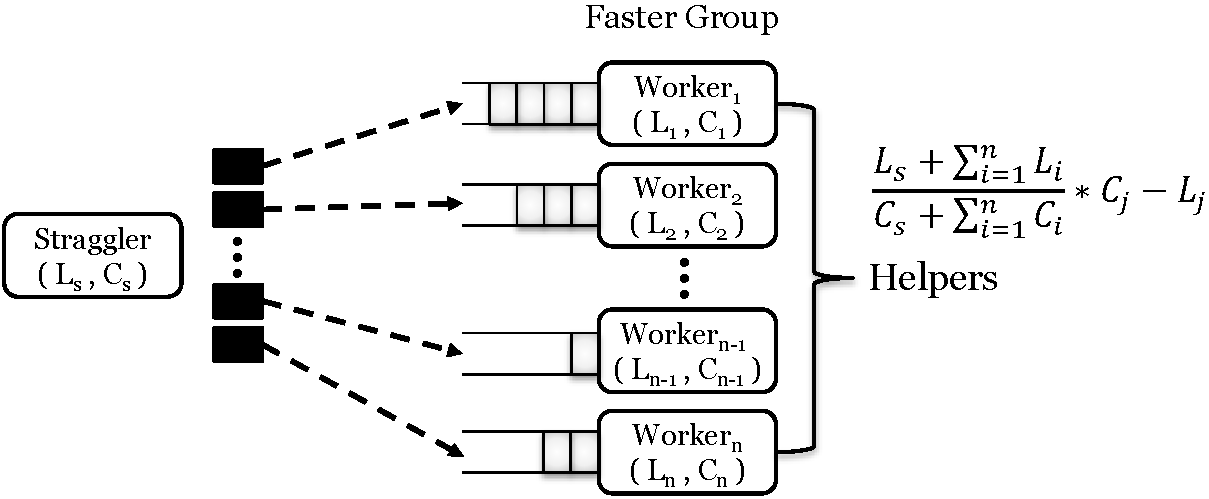
\includegraphics[width=0.48\textwidth]{FigureS1}
    \caption{All Strategy selects all nodes in faster group as helpers.}
    \label{Fig. 8:}
  \end{figure}

  \textbf{Two Choice Strategy.} Different from all strategy, two choice strategy chooses two nodes in faster group as helpers. Lever intends to find out the nodes which have the large computational capability meanwhile have much less input data load as helpers. Fig. 9 shows the principle of two choice strategy. First, Lever sorts the nodes' list according to each node's \emph{$C_i$}/\emph{$L_i$} in the descending order. Then, Lever chooses the head two nodes as helpers and computes load share for each helper. Assume that the selected two nodes have vectors of (\emph{$C_1$},\emph{$L_1$}) and (\emph{$C_2$},\emph{$L_2$}), the straggler can be represented as (\emph{$C_s$},\emph{$L_s$}). The load share \emph{{$L_{sToj}$}} which is dispatched to jth helper can be denoted as:
  \begin{equation}
  L_{sToj} = \frac{L_s + L_1 + L_2}{C_s + C_1 + C_2}*C_j - L_j
  \end{equation}
  After reassignment, Lever updates each node's $C_i$ and $L_i$.
  \begin{figure}[htbp]
    \centering
    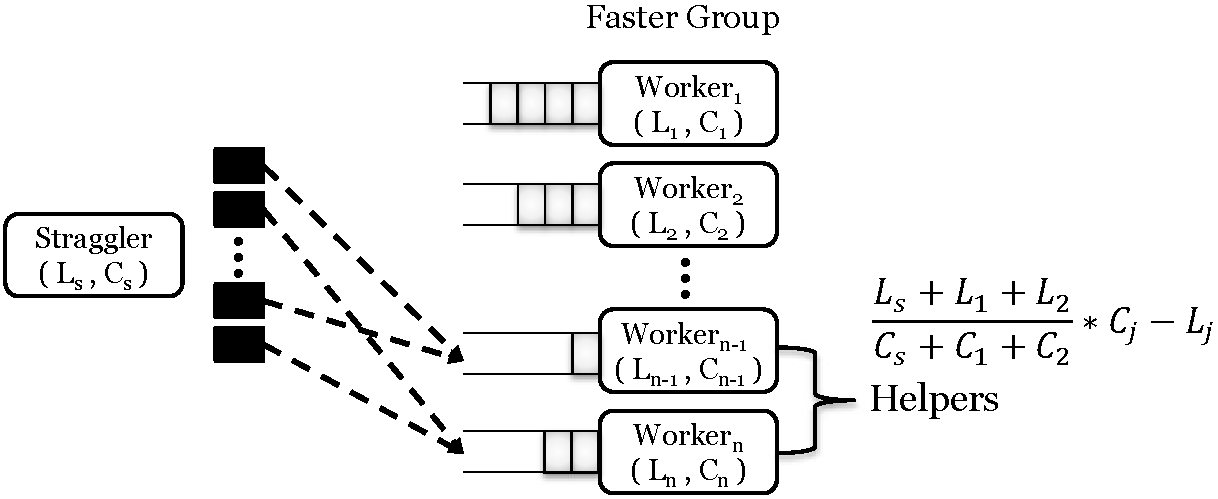
\includegraphics[width=0.48\textwidth]{FigureS2}
    \caption{Two Choice Strategy selects two nodes in faster group as helpers.}
    \label{Fig. 9:}
  \end{figure}

\subsubsection{Adaptively Choose One of Two}

  The above two strategies can be used in different situations. Lever can adaptively choose one of two strategies according to cluster's current state. Obviously, when there are few stragglers, all strategy is much better than two choice strategy because we can pre-schedule input data as evenly as possible. However, if there are more and more stragglers and fasters, two choice strategy will behavior better because of avoiding heavy blocks partition and transmission. Lever combines the latency changes with the \#stragglers$\times$\#fasters to make adaptive choice. If \#stragglers$\times$\#fasters is larger than a observed value, Lever should select two choice strategy. Another case is that Lever uses all strategy last batch, however the applications' latency increases after we pre-scheduling, then Lever will switch to two choice strategy. The complete pseudo code of pre-scheduling algorithm is presented in Algorithm 1.
  \begin{algorithm}[htbp]
  \small
  \caption{Pre-Scheduling Algorithm}
  \label{Alg:1}
  \begin{algorithmic}[1]
  \STATE \textbf{Procedure} \textbf{Identify Potential Stragglers}
  \STATE \quad Get the previous batches' job execution information
  \STATE \quad Sort the nodes descending by their finish time
  \STATE \quad Group the nodes into three groups(straggler, median, faster)
  \STATE \quad Compute the input load's gradient
  \STATE \quad Transform nodes' state according to transition rules
  \STATE \quad Output final stragglers and fasters
  \STATE \textbf{End Procedure}
  \STATE \textbf{Procedure} \textbf{Evaluate Computational Capability}
  \STATE \quad In ith batch, compute i+1th batch's capability
  \STATE \quad $C_{i+1} = C_i + C_i/t_i*(t_{ideal}-t_i)$
  \STATE \quad Assign corresponding load when receiving i+1th batch's data
  \STATE \quad In i+1th batch, compute the next batch's capability
  \STATE \quad $C_{i+2} = C_{i+1} + \frac{C_{i+1}}{t_{i+1}}*(t_{ideal}-t_{i+1})$
  \STATE \textbf{End Procedure}
  \STATE \textbf{Procedure} \textbf{Choose Suitable Helpers and Reassign Work}
  \IF{(\#stragglers$\times$\#fasters$<$$\rho$) or (last batch use AllStrategy \&\& latency decreases)}
  \STATE $/*$ continue to adopt allstrategy $*/$
  \STATE Choose all the nodes as helpers
  \STATE Compute the sum of helpers' capability and the sum of helpers' load
  \STATE $sumOfCapa=\sum_{i=1}^n C_i$ and $sumOfLoad=\sum_{i=1}^n L_i$
  \FOR{each straggler node}
  \FOR{each helper node}
  \STATE Compute the allocated load share
  \STATE $L_{stoi}=\frac{L_s + sumOfLoad}{C_s + sumOfCapa}\times C_i-L_i$
  \STATE Update each node's $(C_i,L_i)$
  \ENDFOR
  \ENDFOR
  \ELSE
  \STATE $/*$ adopt TwoChoiceStrategy $*/$
  \STATE Sort the nodes' list according to each node's $\frac{C_i}{L_i}$ in the descending order
  \STATE Choose the head two nodes as helpers
  \STATE Compute the sum of helpers' capability and the sum of helpers' load
  \STATE $sumOfCapa = C_1 + C_2$ and $sumOfLoad = L_1 + L_2$
  \FOR{each straggler node}
  \FOR{each helper node}
  \STATE Compute the allocated load share
  \STATE $L_{stoi}=\frac{L_s + sumOfLoad}{C_s + sumOfCapa}\times C_i-L_i$
  \STATE Update each node's $(C_i,L_i)$
  \ENDFOR
  \ENDFOR
  \ENDIF
  \STATE \textbf{End Procedure}
  \end{algorithmic}
  \end{algorithm}
